\documentclass[12pt,a4paper,french]{article}

% --- Packages ---
\usepackage[utf8]{inputenc}
\usepackage[T1]{fontenc}
\usepackage[french]{babel}
\usepackage{geometry}
\geometry{margin=2.5cm}
\usepackage{graphicx}
\usepackage{xcolor}
\usepackage{amssymb}
\usepackage{titlesec}
\usepackage[hidelinks]{hyperref}
\usepackage{minted}
\usepackage{tcolorbox}
\tcbuselibrary{minted}
\usepackage{fancyhdr}
\usepackage{charter} 
\usepackage{etoolbox}
\usepackage{pmboxdraw}
\usepackage{forest}
\usepackage[skip=1em]{parskip}
\usepackage{tikz}


% --- Colors ---
\definecolor{primary}{RGB}{0, 75, 135}
\definecolor{secondary}{RGB}{100, 100, 100}

% --- TColorBox Style ---
\tcbset{
    projectbox/.style={
        colback=white,
        colframe=primary!10,
        arc=4pt,
        boxrule=1pt,
        left=10pt,
        right=10pt,
        top=10pt,
        bottom=10pt,
        fonttitle=\bfseries,
        coltitle=primary,
        attach title to upper,
        after title={\medskip\hrule\medskip}
    }
}

% --- Forest Directory Tree Style ---
\forestset{
  dir tree/.style={
    for tree={
      font=\ttfamily,
      grow'=0,
      child anchor=west,
      parent anchor=south,
      anchor=west,
      calign=first,
      edge path={
        \noexpand\path [draw, \forestoption{edge}]
        (!u.south west) +(7.5pt,0) |- node[fill,inner sep=1.25pt] {} (.child anchor)\forestoption{edge label};
      },
      before typesetting nodes={
        if n=1
          {insert before={[,phantom]}}
          {}
      },
      fit=band,
      before computing xy={l=15pt},
    }
  }
}

% --- Setup Minted ---
\setminted{
    style=friendly,
    breaklines=true,
    numbers=none,
    tabsize=2
}

% --- Header/Footer ---
\pagestyle{fancy}
\fancyhf{}
\setlength{\headheight}{15pt}
\lhead{\textcolor{primary}{Projet Micro-Services - Gestion Restaurant}}
\rhead{\thepage}
\lfoot{FSBM - Université Hassan II}

% --- Title Customization ---
\titleformat{\section}{\color{primary}\normalfont\Large\bfseries}{\thesection}{1em}{}
\titleformat{\subsection}{\color{primary}\normalfont\large\bfseries}{\thesubsection}{1em}{}
\titleformat{\subsubsection}{\color{primary}\normalfont\large\bfseries}{\thesubsubsection}{0.5em}{}


% --- Document ---
\begin{document}

% --- Page de Garde ---
\begin{titlepage}
    \centering
    \vspace*{0.5cm}
    
\includegraphics[width=0.6\textwidth]{images/logo.png} \\
    \vspace{1cm}
    {\Large \textbf{Faculté des Sciences Ben M'Sick (FSBM)}}\\[0.5cm]
    {\large Université Hassan II de Casablanca}\\[1.5cm]

    \rule{\linewidth}{0.5mm} \\[0.4cm]
    {\huge \bfseries \textcolor{primary}{Rapport de Projet Micro-Services}} \\[0.2cm]
    {\Large \bfseries Développement d'un Microservice de Gestion de Restaurant} \\
    \rule{\linewidth}{0.5mm} \\[1.5cm]

    \begin{minipage}{0.55\textwidth}
        \begin{flushleft} \large
            \emph{Réalisé par :}\\
            \textbf{Hafssa Bouam} \\
            \textbf{Siham Ait Elmaalem} \\
            \textbf{Hiba Amine} \\
            \textbf{Wiam Armouli} \\
            \textbf{Fatima Zahra Ajmilou} \\
            \textbf{Hafsa ait hmid} \\
            \textbf{Nourelislam Zaitouni} \\
            \textbf{Abdelaziz Taoudi Ebourki} \\
            \textbf{Oussama Rafik}
        \end{flushleft}
    \end{minipage}
    \begin{minipage}{0.35\textwidth}
        \begin{flushright} \large
            \emph{Encadré par :} \\
            \textbf{Pr. CHEMLAL Yman}
        \end{flushright}
    \end{minipage}

    \vfill
    {\large Année Universitaire 2025-2026}
\end{titlepage}

\tableofcontents
\newpage

\section{Introduction}
L'évolution des architectures logicielles vers le modèle microservices est devenue une norme dans l'industrie moderne
du développement. Ce paradigme permet de décomposer une application complexe en un ensemble de services petits,
autonomes et communicants via des protocoles légers. Cette approche facilite non seulement la maintenance
et le déploiement continu, mais offre également une scalabilité granulaire indispensable aux applications industrielles.

Dans le cadre du module \textbf{Micro-Services}, notre équipe a été chargée de concevoir et réaliser un microservice
autonome pour la gestion de la carte d'un restaurant. Ce service est construit sur l'écosystème \textit{Spring Boot}
et respecte les principes fondamentaux du style architectural \textit{REST}.

Ce rapport présente les étapes clés de la réalisation de ce projet, depuis la conception architecturale jusqu'à
la mise en \oe{}uvre technique. Nous détaillerons la structure du projet, l'implémentation des différentes couches
logicielles, ainsi que les phases de validation et de test.

\section{Cahier des Charges}
\subsection{Objectifs du Projet}
L'objectif principal est de fournir une solution robuste pour la gestion des plats d'un restaurant. Le système doit
permettre aux gestionnaires de manipuler la carte de manière intuitive tout en garantissant l'intégrité des
données métiers. L'utilisation de \textit{Spring Boot} a été imposée pour sa capacité à produire des applications
``production-ready'' avec un minimum de configuration manuelle.

\subsection{Exigences Fonctionnelles}
Le microservice doit supporter l'ensemble des opérations \textit{CRUD} (Create, Read, Update, Delete) sur la
ressource \mintinline{java}{Plat} :
\begin{itemize}
    \item \textbf{Ajout} : Insertion de nouveaux plats via \texttt{POST} avec validation des prix.
    \item \textbf{Consultation} : Récupération globale ou spécifique par identifiant unique (\texttt{ID}).
    \item \textbf{Mise à jour} : Modification des propriétés d'un plat existant via \texttt{PUT}.
    \item \textbf{Suppression} : Retrait définitif d'un plat via \texttt{DELETE}.
    \item \textbf{Recherche Métier} : Un endpoint spécifique pour filtrer les plats ``Healthy'' (moins de 500 calories).
\end{itemize}

\subsection{Contraintes Techniques}
\begin{itemize}
    \item \textbf{Persistence} : Utilisation de \textit{Spring Data JPA} avec une base de données \textit{H2} en
          mémoire pour la rapidité des tests.
    \item \textbf{Architecture} : Respect strict du modèle \textit{MVC} et injection de dépendances par constructeur.
    \item \textbf{Sécurité} : Masquage du coût des ingrédients dans les réponses API pour des raisons de
          confidentialité métier.
    \item \textbf{Documentation} : Interface \textit{Swagger} interactive pour faciliter l'intégration par des tiers.
\end{itemize}

\section{Conception et Architecture}
\subsection{Analyse de la Structure}
Le projet suit une structure modulaire standardisée. Cette séparation des préoccupations (\textit{Separation of Concerns})
permet à chaque membre de l'équipe de travailler sur une couche spécifique sans interférer avec les autres.

\begin{tcolorbox}[projectbox, title=Arborescence du Projet]
    \begin{forest}
        dir tree
        [restaurant/
        [src/
        [main/
        [java/
        [com.restaurant.restaurant/
        [RestaurantApplication.java]
        [dao/
        [PlatRepository.java]
        ]
        [model/
        [Plat.java]
        ]
        [web/
        [controller/
        [PlatController.java]
        ]
        [exceptions/
        [GlobalExceptionHandler.java]
        [ResourceNotFoundException.java]
        ]
        ]
        ]
        ]
        [resources/
        [application.properties]
        [schema.sql]
        [data.sql]
        ]
        ]
        ]
        [pom.xml]
        ]
    \end{forest}
\end{tcolorbox}

\subsection{Schéma Architectural}
L'architecture du microservice suit une approche modulaire permettant de découpler
la logique métier des interfaces techniques (API) et de la persistance.

\begin{tcolorbox}[projectbox, title=Flux de Données et Composants]
    \centering
    \begin{tikzpicture}[node distance=2.5cm, auto, >=stealth]
        % Styles
        \tikzset{external/.style={rectangle, draw=primary!50, fill=primary!5, text width=2.5cm, text centered, rounded corners, minimum height=1cm}}
        \tikzset{port/.style={rectangle, draw=primary!80, fill=primary!10, text width=2cm, text centered, rounded corners, minimum height=0.8cm}}
        \tikzset{core/.style={rectangle, draw=primary, fill=primary!20, text width=2.5cm, text centered, rounded corners, minimum height=1cm}}

        % Actors
        \node[external] (client) {Client HTTP};
        \node[external, below of=client] (database) {Base H2};

        % Ports
        \node[port, right of=client, xshift=2.5cm] (rest) {API REST};
        \node[port, right of=database, xshift=2.5cm] (persistence) {Persistance};

        % Core
        \node[core, right of=rest, xshift=2.5cm] (controller) {Contrôleur};
        \node[core, below of=controller] (repository) {Repository};

        % Connections
        \draw[->, thick] (client) -- (rest);
        \draw[->, thick] (rest) -- (controller);
        \draw[<->, thick] (controller) -- (repository);
        \draw[->, thick] (repository) -- (persistence);
        \draw[->, thick] (persistence) -- (database);
    \end{tikzpicture}
\end{tcolorbox}

\subsection{Modélisation de la Ressource}
L'entité \mintinline{java}{Plat} est le c\oe{}ur de notre domaine. Elle utilise les annotations \textit{JPA} pour
le mapping relationnel et \textit{Jackson} pour le contrôle de la sérialisation \texttt{JSON}.

\begin{tcolorbox}[projectbox, title=Plat.java]
    \begin{minted}{java}
@Entity
public class Plat {
    @Id
    @GeneratedValue(strategy = GenerationType.IDENTITY)
    private Long id;

    @NotBlank(message = "Le nom du plat est obligatoire")
    private String nom;

    private int calories;

    @Positive(message = "Le prix doit être positif")
    private double prix;

    @JsonProperty(access = JsonProperty.Access.WRITE_ONLY)
    private double coutIngredients;

    public Plat() {}

    public Plat(String nom, int calories, double prix, double coutIngredients) {
        this.nom = nom;
        this.calories = calories;
        this.prix = prix;
        this.coutIngredients = coutIngredients;
    }
}
\end{minted}
\end{tcolorbox}

\section{Mise en \OE{}uvre Technique}
\subsection{Configuration de l'Application}
Le fichier \texttt{application.properties} définit le comportement de la base de données \textit{H2} et du moteur
\textit{Hibernate}. Nous avons activé le mode \texttt{defer-datasource-initialization} pour garantir que les scripts
\texttt{SQL} s'exécutent après la création des tables par \textit{JPA}.

\begin{tcolorbox}[projectbox, title=application.properties]
    \begin{minted}{properties}
spring.datasource.url=jdbc:h2:mem:restaurantdb
spring.h2.console.enabled=true
spring.h2.console.path=/h2-console

spring.jpa.hibernate.ddl-auto=none
spring.jpa.defer-datasource-initialization=true
spring.sql.init.mode=always
spring.jpa.show-sql=true
\end{minted}
\end{tcolorbox}

\subsection{Couche DAO et Persistance}
Le repository utilise l'interface \mintinline{java}{JpaRepository} qui fournit par défaut toutes les méthodes
\textit{CRUD}. Nous y avons ajouté une méthode de requête dérivée (\textit{Query Method}) pour le filtrage par calories.

\begin{tcolorbox}[projectbox, title=PlatRepository.java]
    \begin{minted}{java}
@Repository
public interface PlatRepository extends JpaRepository<Plat, Long> {
    List<Plat> findByCaloriesLessThan(int maxCalories);
}
\end{minted}
\end{tcolorbox}

\subsection{Initialisation des Données (SQL)}
Pour assurer la portabilité et faciliter les tests, nous utilisons deux fichiers \texttt{SQL} chargés
automatiquement au démarrage.

\begin{tcolorbox}[projectbox, title=schema.sql]
    \begin{minted}{sql}
CREATE TABLE plat (
    id BIGINT AUTO_INCREMENT PRIMARY KEY,
    nom VARCHAR(100) NOT NULL,
    calories INT NOT NULL,
    prix DOUBLE NOT NULL,
    cout_ingredients DOUBLE NOT NULL
);
\end{minted}
\end{tcolorbox}

\begin{tcolorbox}[projectbox, title=data.sql]
    \begin{minted}{sql}
INSERT INTO plat (nom, calories, prix, cout_ingredients) VALUES 
('Salade César', 350, 12.50, 4.20),
('Burger Gourmet', 850, 18.00, 7.50),
('Poke Bowl Saumon', 450, 14.00, 6.00);
\end{minted}
\end{tcolorbox}

\subsection{Couche Contrôleur REST}
La classe \mintinline{java}{PlatController} orchestre les requêtes entrantes. Elle délègue la persistance
au repository et assure la transformation des données en réponses HTTP.

\begin{tcolorbox}[projectbox, title=Signature de PlatController.java]
    \begin{minted}{java}
@RestController
@RequestMapping("/plats")
public class PlatController {
    private final PlatRepository platRepository;

    public PlatController(PlatRepository platRepository);
    public List<Plat> listePlats();
    public Plat getPlatById(Long id);
    public List<Plat> getPlatsHealthy();
    public ResponseEntity<Plat> ajouterPlat(Plat plat);
    public ResponseEntity<Plat> modifierPlat(Long id, Plat platDetails);
    public ResponseEntity<Void> deletePlat(Long id);
}
\end{minted}
\end{tcolorbox}

\subsubsection{Détails des méthodes}

\textbf{Injection de dépendances}
\begin{minted}{java}
public PlatController(PlatRepository platRepository) {
    this.platRepository = platRepository;
}
\end{minted}
Le constructeur garantit que le contrôleur dispose toujours d'une instance valide du repository pour
interagir avec la base de données.

\vspace{1em}
\textbf{Récupération globale}
\begin{minted}{java}
@GetMapping
public List<Plat> listePlats() {
    return platRepository.findAll();
}
\end{minted}
Cette méthode récupère l'intégralité des plats via la méthode standard \texttt{findAll()} de Spring Data JPA.

\vspace{1em}
\textbf{Récupération par identifiant}
\begin{minted}{java}
@GetMapping("/{id}")
public Plat getPlatById(@PathVariable Long id) {
    return platRepository.findById(id)
            .orElseThrow(() -> new ResourceNotFoundException("Plat non trouvé avec id : " + id));
}
\end{minted}
Permet de consulter un plat spécifique. En cas d'absence, elle lève une exception
\mintinline{java}{ResourceNotFoundException}.

\vspace{1em}
\textbf{Filtre métier Healthy}
\begin{minted}{java}
@GetMapping("/healthy")
public List<Plat> getPlatsHealthy() {
    return platRepository.findByCaloriesLessThan(500);
}
\end{minted}
Implémente le filtrage des plats considérés comme sains (moins de 500 calories).

\vspace{1em}
\textbf{Création de ressource}
\begin{minted}{java}
@PostMapping
public ResponseEntity<Plat> ajouterPlat(@Valid @RequestBody Plat plat) {
    Plat platAjoute = platRepository.save(plat);
    return new ResponseEntity<>(platAjoute, HttpStatus.CREATED);
}
\end{minted}
Gère l'ajout d'un plat avec validation des données et retourne un code \texttt{201 Created}.

\vspace{1em}
\textbf{Mise à jour complète}
\begin{minted}{java}
@PutMapping("/{id}")
public ResponseEntity<Plat> modifierPlat(@PathVariable Long id, @Valid @RequestBody Plat platDetails) {
    Plat plat = platRepository.findById(id)
            .orElseThrow(() -> new ResourceNotFoundException("Plat non trouvé avec id : " + id));

    plat.setNom(platDetails.getNom());
    plat.setCalories(platDetails.getCalories());
    plat.setPrix(platDetails.getPrix());
    plat.setCoutIngredients(platDetails.getCoutIngredients());

    return ResponseEntity.ok(platRepository.save(plat));
}
\end{minted}
Met à jour une ressource existante après avoir vérifié son existence.

\vspace{1em}
\textbf{Suppression de ressource}
\begin{minted}{java}
@DeleteMapping("/{id}")
public ResponseEntity<Void> deletePlat(@PathVariable Long id) {
    if (!platRepository.existsById(id)) {
        throw new ResourceNotFoundException("Plat non trouvé avec id : " + id);
    }
    platRepository.deleteById(id);
    return ResponseEntity.noContent().build();
}
\end{minted}
Supprime un plat et renvoie un code \texttt{204 No Content}.

\subsection{Gestion Globale des Exceptions}
Le \mintinline{java}{GlobalExceptionHandler} centralise le traitement des erreurs pour garantir des réponses
JSON uniformes.

\begin{tcolorbox}[projectbox, title=Signature de GlobalExceptionHandler.java]
    \begin{minted}{java}
@ControllerAdvice
public class GlobalExceptionHandler {
    public ResponseEntity<Object> handleResourceNotFoundException(ResourceNotFoundException ex);
    public ResponseEntity<Object> handleValidationExceptions(MethodArgumentNotValidException ex);
    public ResponseEntity<Object> handleNoResourceFound(NoResourceFoundException ex);
    public ResponseEntity<Object> handleGlobalException(Exception ex);
}
\end{minted}
\end{tcolorbox}

\subsubsection{Traitement des erreurs spécifiques}

\textbf{Ressource non trouvée (404)}
\begin{minted}{java}
@ExceptionHandler(ResourceNotFoundException.class)
public ResponseEntity<Object> handleResourceNotFoundException(ResourceNotFoundException ex) {
    Map<String, Object> body = new HashMap<>();
    body.put("timestamp", LocalDateTime.now());
    body.put("message", ex.getMessage());
    body.put("status", HttpStatus.NOT_FOUND.value());
    return new ResponseEntity<>(body, HttpStatus.NOT_FOUND);
}
\end{minted}

\vspace{1em}
\textbf{Erreurs de validation (400)}
\begin{minted}{java}
@ExceptionHandler(MethodArgumentNotValidException.class)
public ResponseEntity<Object> handleValidationExceptions(MethodArgumentNotValidException ex) {
    Map<String, Object> errors = new HashMap<>();
    ex.getBindingResult().getFieldErrors()
            .forEach(error -> errors.put(error.getField(), error.getDefaultMessage()));

    Map<String, Object> body = new HashMap<>();
    body.put("timestamp", LocalDateTime.now());
    body.put("errors", errors);
    body.put("status", HttpStatus.BAD_REQUEST.value());
    return new ResponseEntity<>(body, HttpStatus.BAD_REQUEST);
}
\end{minted}

\vspace{1em}
\textbf{URL non trouvée (404)}
\begin{minted}{java}
@ExceptionHandler(NoResourceFoundException.class)
public ResponseEntity<Object> handleNoResourceFound(NoResourceFoundException ex) {
    Map<String, Object> body = new HashMap<>();
    body.put("timestamp", LocalDateTime.now());
    body.put("message", "Endpoint non trouvé");
    body.put("status", HttpStatus.NOT_FOUND.value());
    return new ResponseEntity<>(body, HttpStatus.NOT_FOUND);
}
\end{minted}

\vspace{1em}
\textbf{Sécurité par défaut (500)}
\begin{minted}{java}
@ExceptionHandler(Exception.class)
public ResponseEntity<Object> handleGlobalException(Exception ex) {
    Map<String, Object> body = new HashMap<>();
    body.put("timestamp", LocalDateTime.now());
    body.put("message", "Une erreur interne s'est produite.");
    body.put("status", HttpStatus.INTERNAL_SERVER_ERROR.value());
    return new ResponseEntity<>(body, HttpStatus.INTERNAL_SERVER_ERROR);
}
\end{minted}

\section{Validation et Tests}
\subsection{Documentation Interactive}
Grâce à \textit{SpringDoc OpenAPI}, notre API s'auto-documente. En accédant à \texttt{/swagger-ui/index.html},
les développeurs peuvent visualiser les schémas de données et tester les requêtes sans outils tiers.

\subsection{Suite de Tests Postman}
Une collection \textit{Postman} a été créée pour automatiser la validation des exigences. Chaque requête inclut
des scripts de test en \textit{JavaScript} pour vérifier les codes de retour et la structure du \texttt{JSON}.

\begin{tcolorbox}[projectbox, title=Collection Postman (Extraits)]
    \begin{minted}{json}
{
  "name": "Ajouter Plat",
  "request": {
    "method": "POST",
    "url": "http://localhost:8080/plats",
    "body": { "mode": "raw", "raw": "{\"nom\": \"Salade César\", \"calories\": 450, \"prix\": 12.0}" }
  },
  "event": [ {
      "listen": "test",
      "script": { "exec": [
          "pm.test('Status est 201', function () { pm.response.to.have.status(201); });",
          "pm.test('Filtrage JSON : coutIngredients absent', function () { ",
          "    pm.expect(pm.response.json().coutIngredients)
          .to.be.undefined; });"
      ] }
  } ]
}
\end{minted}
\end{tcolorbox}

\subsection{Résultats des Tests (Validation)}

\begin{tcolorbox}[projectbox, title=Console H2 : État de la Base de Données]
    \centering
    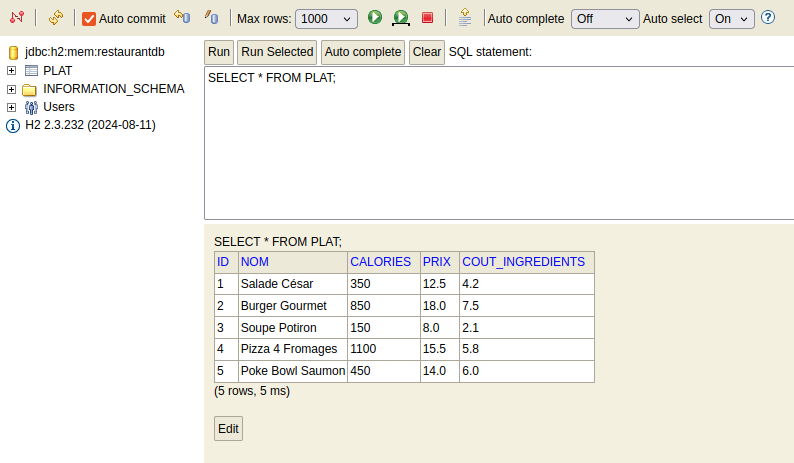
\includegraphics[width=0.9\textwidth]{images/h2_console.png}
\end{tcolorbox}
La console H2 permet de visualiser en temps réel l'état de la base de données relationnelle en
mémoire. Comme illustré ci-dessus, les tables sont correctement générées par Hibernate, et les
données initiales définies dans le fichier \texttt{data.sql} sont bien présentes, confirmant le
bon fonctionnement de la couche de persistance dès le démarrage.

\begin{tcolorbox}[projectbox, title=Documentation API (Swagger UI)]
    \centering
    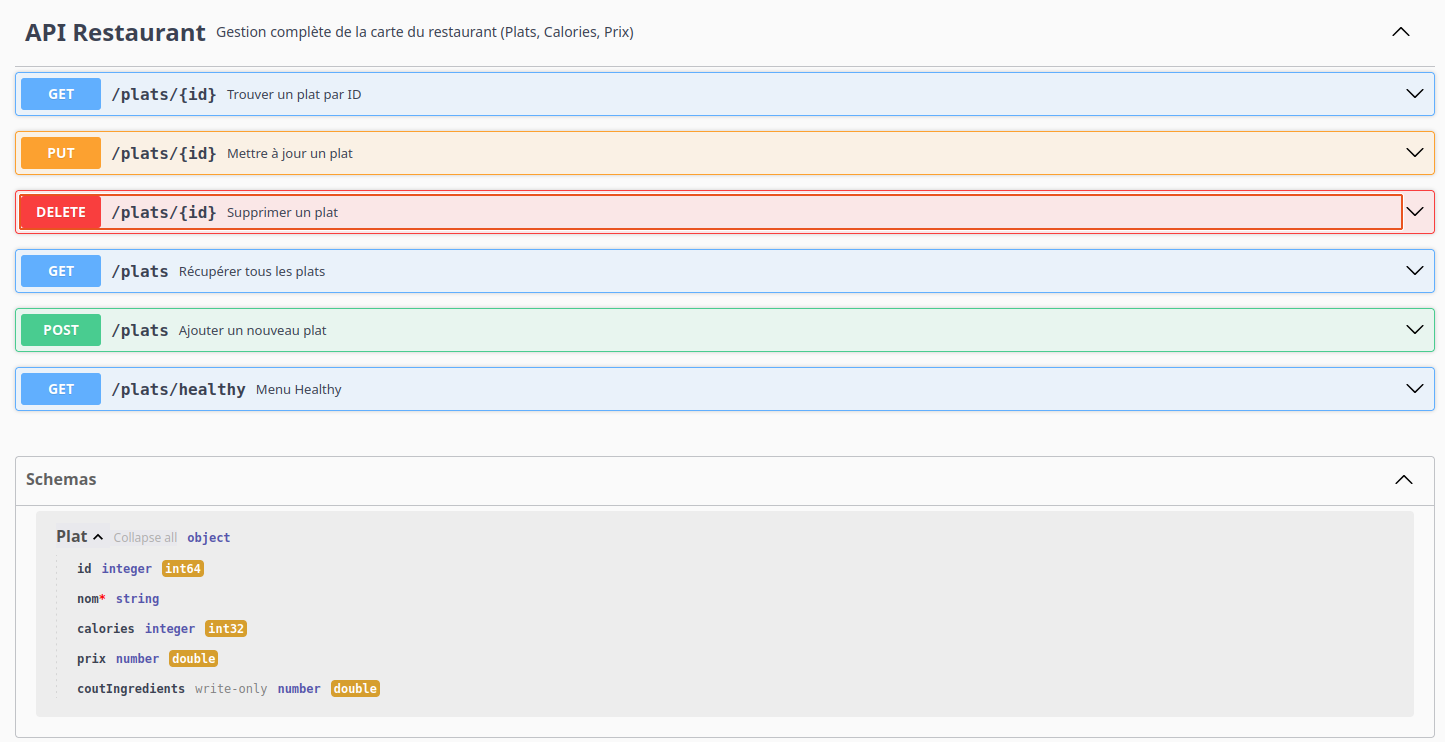
\includegraphics[width=0.9\textwidth]{images/swagger_ui.png}
\end{tcolorbox}
L'interface Swagger UI offre une vue exhaustive de tous les points d'accès (endpoints) exposés par
le microservice. Elle permet non seulement de consulter les schémas de données attendus pour
chaque requête, mais aussi d'exécuter des tests interactifs directement depuis le navigateur,
facilitant ainsi grandement le travail d'intégration pour les clients de l'API.

\begin{tcolorbox}[projectbox, title=Test : Ajout d'un Plat (Succès 201)]
    \small\textbf{Requête}
    \begin{minted}{http}
POST /plats HTTP/1.1
Content-Type: application/json
\end{minted}
    \begin{minted}{json}
{
  "nom": "Pasta Pesto",
  "calories": 450,
  "prix": 14.5,
  "coutIngredients": 4.0
}
\end{minted}
    \small\textbf{Réponse}
    \begin{minted}{http}
HTTP/1.1 201 Created
\end{minted}
    \begin{minted}{json}
{
  "id": 7,
  "nom": "Pasta Pesto",
  "calories": 450,
  "prix": 14.5
}
\end{minted}
\end{tcolorbox}
Cette interaction démontre la création d'une ressource. On observe que l'API retourne un code
\texttt{201 Created}. Conformément aux exigences, le champ \texttt{coutIngredients} envoyé
dans la requête est bien masqué dans la réponse JSON, protégeant les données de coût.

\begin{tcolorbox}[projectbox, title=Test : Recherche Métier Healthy (Calories < 500)]
    \small\textbf{Requête}
    \begin{minted}{http}
GET /plats/healthy HTTP/1.1
\end{minted}
    \small\textbf{Réponse}
    \begin{minted}{http}
HTTP/1.1 200 OK
\end{minted}
    \begin{minted}{json}
[
  { "id": 1, "nom": "Salade César", "calories": 350, "prix": 12.5 },
  { "id": 3, "nom": "Soupe Potiron", "calories": 150, "prix": 8.0 },
  { "id": 5, "nom": "Poke Bowl Saumon", "calories": 450, "prix": 14.0 },
  { "id": 7, "nom": "Pasta Pesto", "calories": 450, "prix": 14.5 }
]
\end{minted}
\end{tcolorbox}
L'appel au endpoint dédié au menu ``Healthy'' confirme l'efficacité du filtrage. Le serveur
renvoie exclusivement les plats dont l'apport calorique est inférieur au seuil de 500 calories,
validant l'implémentation de la requête dérivée dans la couche DAO.

\begin{tcolorbox}[projectbox, title=Test : Validation des Données (Erreur 400)]
    \small\textbf{Requête}
    \begin{minted}{http}
POST /plats HTTP/1.1
\end{minted}
    \begin{minted}{json}
{ 
  "nom": "", 
  "prix": -10 
}
\end{minted}
    \small\textbf{Réponse}
    \begin{minted}{http}
HTTP/1.1 400 Bad Request
\end{minted}
    \begin{minted}{json}
{
  "status": 400,
  "errors": {
    "prix": "Le prix doit être positif",
    "nom": "Le nom du plat est obligatoire"
  },
  "timestamp": "2026-03-26T16:55:53.790"
}
\end{minted}
\end{tcolorbox}
L'envoi de données invalides déclenche immédiatement une erreur \texttt{400 Bad Request}.
Le dictionnaire d'erreurs renvoyé par le \mintinline{java}{GlobalExceptionHandler} permet
au client de corriger précisément les champs posant problème (nom vide et prix négatif).

\begin{tcolorbox}[projectbox, title=Test : Ressource non trouvée (Erreur 404)]
    \small\textbf{Requête}
    \begin{minted}{http}
GET /plats/999 HTTP/1.1
\end{minted}
    \small\textbf{Réponse}
    \begin{minted}{http}
HTTP/1.1 404 Not Found
\end{minted}
    \begin{minted}{json}
{
  "status": 404,
  "message": "Plat non trouvé avec id : 999",
  "timestamp": "2026-03-26T16:56:33.915"
}
\end{minted}
\end{tcolorbox}
La gestion des identifiants inexistants est illustrée ici. Le service répond par un code
\texttt{404 Not Found} standard, accompagné d'un message explicatif, assurant une gestion
robuste des exceptions métier à travers toute l'application.

\section{Gestion du Projet}
La répartition des tâches a permis une progression quasi parallèle:
\begin{itemize}
    \item \textbf{Architecture} : Configuration initiale, \textit{Maven}, dépendances et structure.
    \item \textbf{Conception} : Modèle de données et règles de validation.
    \item \textbf{Data Access} : Scripts \texttt{SQL} et couche de persistance.
    \item \textbf{Contrôleur} : Implémentation des endpoints \texttt{GET} et \texttt{POST}.
    \item \textbf{Logique Métier} : Développement de la logique métier ``Healthy''.
    \item \textbf{Mise à jour} : Implémentation de la méthode \texttt{PUT} pour les modifications.
    \item \textbf{Suppression} : Gestion de la suppression et des codes \textit{No Content}.
    \item \textbf{Sécurité et Exceptions} : Sécurisation via le gestionnaire d'exceptions.
    \item \textbf{Documentation et Tests} : Documentation \textit{Swagger} et tests \textit{Postman}.
\end{itemize}

\section{Conclusion}
En conclusion, ce projet a permis de concevoir et d'implémenter un microservice de gestion
de restaurant complet, respectant rigoureusement les standards industriels actuels.
L'architecture adoptée, reposant sur \textit{Spring Boot} et \textit{Spring Data JPA},
garantit une séparation claire des responsabilités et une persistance des données
efficace via une base \textit{H2} en mémoire.

L'intégration de \textit{Bean Validation} et d'un gestionnaire global d'exceptions a
renforcé la robustesse du système, tandis que l'utilisation de \textit{Jackson} pour
le filtrage \texttt{JSON} a assuré la confidentialité des données sensibles comme
le coût des ingrédients. Enfin, l'exposition d'une documentation interactive via
\textit{Swagger} et la validation par une suite de tests \textit{Postman} rigoureuse
confirment la qualité et la conformité du service aux exigences du cahier des charges.

\end{document}
